%%
%% This is file `sample-sigconf-authordraft.tex',
%%
%%
\documentclass[sigconf, screen, review, anonymous]{acmart}

%% BibTeX command
\AtBeginDocument{%
  \providecommand\BibTeX{{%
    Bib\TeX}}}

%% Rights management information (placeholder)
\setcopyright{acmlicensed}
\copyrightyear{2026}
\acmYear{2026}
\acmDOI{XXXXXXX.XXXXXXX}
\acmConference[ACMMM '26]{ACM Multimedia 2026}{October 2026}{TBD}
\acmISBN{978-1-4503-XXXX-X/2026/10}

%% Additional packages
\usepackage{amsmath}
\usepackage{algorithm}
\usepackage{algorithmic}
\usepackage{multirow}
\usepackage{subcaption}
\usepackage{cleveref}

%% Custom math operators
\DeclareMathOperator{\sigmoid}{sigmoid}
\newcommand{\bx}{\mathbf{x}}
\newcommand{\bc}{\mathbf{c}}
\newcommand{\bz}{\mathbf{z}}
\newcommand{\bm}{\mathbf{m}}
\newcommand{\btau}{\boldsymbol{\tau}}
\newcommand{\etal}{\textit{et~al.}}

%%
%% end of the preamble, start of the body of the document source.
\begin{document}


\title{CRR-Flow: State-Aware Autoregressive Flow for Long-Horizon Human-Object Interaction Generation}

\author{First Author}
\email{first@institution.edu}
\affiliation{%
  \institution{Institution}
  \city{City}
  \country{Country}
}

\author{Second Author}
\email{second@institution.edu}
\affiliation{%
  \institution{Institution}
  \city{City}
  \country{Country}
}

\author{Third Author}
\email{third@institution.edu}
\affiliation{%
  \institution{Institution}
  \city{City}
  \country{Country}
}

\renewcommand{\shortauthors}{First Author et al.}


%%
%% Abstract
%%
\begin{abstract}



Synthesizing long-horizon 3D human-object interactions (HOI) in which a person manipulates multiple objects across a continuous sequence of phases is an open problem.
% While recent generative models have shown promise in short-term HOI synthesis, they struggle to maintain temporal continuity and physical coherence in multi-step, extended tasks. Specifically, current methods typically generate motion primitives independently from a rest pose, which fails to model the evolving state-dependent correspondence between hands and various objects. This leads to abrupt transitions at primitive boundaries and a loss of hand-object contact consistency over long durations.
Current generative approaches produce motion primitives independently, typically resetting from a canonical rest pose, and therefore cannot model the evolving correspondence between the human body and objects as physical states change. This results in abrupt transitions at primitive boundaries and a progressive loss of contact consistency over extended horizons.
We present CRR-Flow (Contact-Reach-Release Flow), a framework that couples high-level task planning with state-aware motion synthesis via conditional flow matching.
An LLM-based planner first decomposes multi-step instructions into per-slot physical state schedules, assigning a discrete interaction phase to each interaction component (body, hands, and objects) over contiguous temporal segments.
% Entity --> slot
%We then propose an entity-centric Diffusion Transformer that models the body, hands, and objects as dedicated spatial tokens, enabling the precise routing of scheduled interaction constraints.
These schedules condition a slot-centric Diffusion Transformer whose dedicated spatial tokens per interaction component allow each to receive its own state and geometry information.
A block-wise autoregressive strategy in which each generation block is conditioned on the terminal kinematic history of the previous block, propagating position and velocity across primitive boundaries.
% 细节就不需要了
% To preserve geometric fidelity, static object shape is encoded via Basis Point Set (BPS) descriptors and supplied as clean context, so that flow-matching noise acts only on dynamic kinematics.
% 实验结果最后更新一版然后在这里可以强调一下improve的百分比
Experiments on OakInk2 show that CRR-Flow reduces FID by 84.5\% relative to InterAct HOIDiff (0.438 vs.\ 2.821) and achieves long-horizon generation over 60+ seconds with only 8.6\% degradation from single-segment quality. Contact evaluation on GRAB confirms that per-slot state 
injection nearly doubles Contact F1 (0.251 vs.\ 0.129).
\end{abstract}

% \begin{abstract}








% Experiments on OakInk2, GRAB, and OMOMO show that CRR-Flow reduces reconstruction error by over 30\% relative to a non-autoregressive variant and maintains coherent generation across multi-segment chains, outperforming existing baselines in both contact consistency and motion smoothness.
% \end{abstract}


%%
%% CCS Concepts
%%
\begin{CCSXML}
<ccs2012>
   <concept>
       <concept_id>10010147.10010371.10010352.10010380</concept_id>
       <concept_desc>Computing methodologies~Motion processing</concept_desc>
       <concept_significance>500</concept_significance>
       </concept>
   <concept>
       <concept_id>10010147.10010257.10010293.10010294</concept_id>
       <concept_desc>Computing methodologies~Neural networks</concept_desc>
       <concept_significance>500</concept_significance>
       </concept>
   <concept>
       <concept_id>10010147.10010371.10010352</concept_id>
       <concept_desc>Computing methodologies~Animation</concept_desc>
       <concept_significance>300</concept_significance>
       </concept>
 </ccs2012>
\end{CCSXML}

\ccsdesc[500]{Computing methodologies~Motion processing}
\ccsdesc[500]{Computing methodologies~Neural networks}
\ccsdesc[300]{Computing methodologies~Animation}


%%
%% Keywords
%%
\keywords{Human-object interaction, motion generation, flow matching, long-term synthesis, text-driven generation.}



%%
%% Teaser figure
%%
\begin{teaserfigure}
  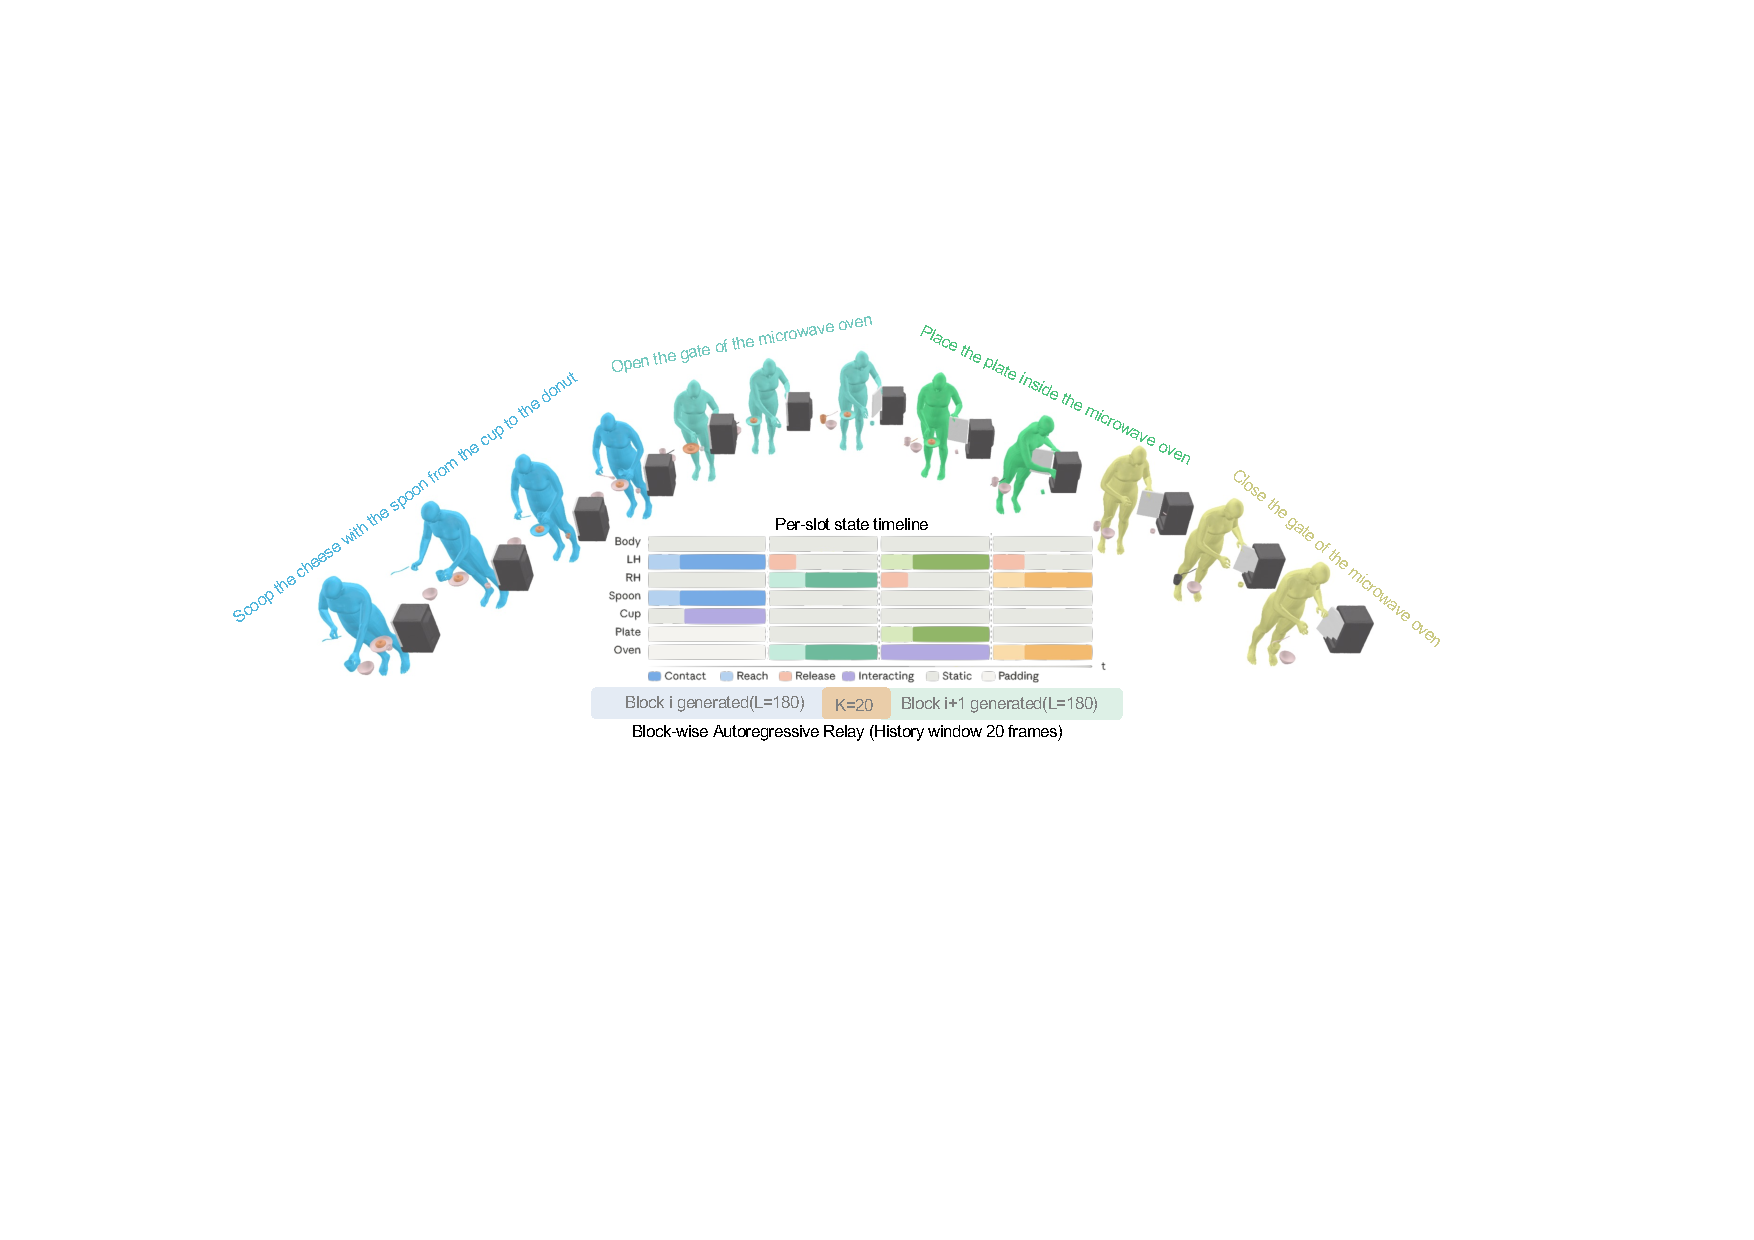
\includegraphics[width=\textwidth]{./figures/tease.pdf}
  \caption{\textbf{CRR-Flow generates long-horizon, multi-object manipulation from multi-step instructions.}
  Given four consecutive primitive instructions, an LLM-based planner produces a per-slot state timeline (center) that assigns a discrete interaction phase (Reach, Contact, Release, Interacting, or Static) to each slot---body, hands, and objects.
  A slot-centric Diffusion Transformer then synthesizes motion within each generation block, while a block-wise autoregressive relay (bottom) propagates the last 20 frames of each block as kinematic history for the next, maintaining continuous dynamics across segment boundaries.
  The resulting sequence spans four primitives with coordinated bimanual manipulation of multiple objects.}
  \Description{A long-horizon manipulation sequence generated by CRR-Flow, showing four color-coded segments: scooping cheese with a spoon (blue), opening a microwave oven gate (teal), placing a plate inside the oven (green), and closing the oven gate (yellow). The center displays a per-slot state timeline matrix with rows for body, left hand, right hand, spoon, cup, plate, and oven, where each cell is colored by interaction phase. Below, a block-wise autoregressive relay diagram shows how consecutive generation blocks overlap by a 20-frame history window to ensure temporal continuity.}
  \label{fig:tease}
\end{teaserfigure}

\maketitle


%% ============================================================
%% 1. INTRODUCTION
%% ============================================================
\section{Introduction}
\label{sec:intro}

Long-horizon 3D human-object interaction (HOI) synthesis aims to produce physically plausible and temporally coherent motion sequences from complex, multi-step natural language instructions.
This capability is central to robotic manipulation planning, virtual reality, and character animation.

Text-driven motion synthesis has advanced rapidly. Diffusion-based methods such as MDM~\cite{tevet2023human}, MLD~\cite{chen2023executing}, and MotionDiffuse~\cite{zhang2022motiondiffuse} generate diverse, high-quality body motions, while T2M-GPT~\cite{zhang2023t2mgpt} and MoMask~\cite{guo2024momask} explore discrete tokenization for motion generation. 
In HOI synthesis, InterAct~\cite{xu2025interact} consolidates large-scale HOI data with a unified framework, and datasets such as GRAB~\cite{taheri2020grab} and OakInk2~\cite{zhan2024oakink2} provide rich annotations for interactions. 
However, these interaction methods are confined to single-instruction, single-object scenarios, generating fixed-length clips that capture only one primitive action at a time. They fail to model how the correspondence between human and multiple objects evolves throughout an extended task, for instance, that the right hand must release a bottle cap before the left hand can begin pouring. 
Separately, long-term body motion composition methods, such as TEACH~\cite{athanasiou2022teach} and PriorMDM~\cite{shafir2024priormdm}, address temporal extension by stitching body motion segments. Yet, these methods operate exclusively on body-only motion without modeling contact physics or object dynamics. As a result, \textit{no existing method can generate long-horizon HOI from multi-step instructions while maintaining both physical plausibility and temporal coherence across primitive boundaries.}
% Consider the task of preparing a cup of tea: a person must unscrew the bottle cap with one hand while stabilizing the bottle with the other, pour water into the cup, set the bottle down, pick up a spoon, and stir.
% Executing this task requires synthesizing a manipulation sequence that spans thousands of frames, coordinates both hands with multiple objects through successive contact phases, and maintains physical plausibility not only within each primitive action but also across the transitions between them.
% Generating such long-horizon, multi-object hand-object interactions from natural language instructions is a fundamental capability for applications in robotics, character animation, virtual reality, and assistive technology, yet it remains largely unsolved.

% Recent years have witnessed significant progress in text-driven motion synthesis.
% Diffusion-based methods such as MDM~\cite{tevet2023human}, MLD~\cite{chen2023executing}, and MotionDiffuse~\cite{zhang2022motiondiffuse} generate diverse, high-quality body motions from short text prompts, while T2M-GPT~\cite{zhang2023t2mgpt} and MoMask~\cite{guo2024momask} explore discrete tokenization for motion generation.
% In the hand-object interaction domain, DiffH2O~\cite{christen2024diffh2o} introduces a two-phase diffusion pipeline for grasping and manipulation, InterAct~\cite{xu2025interact} consolidates large-scale HOI data with a unified generative framework, and datasets such as GRAB~\cite{taheri2020grab} and OakInk2~\cite{zhan2024oakink2} provide rich annotations for bimanual manipulation with multiple objects.
% However, these interaction methods are confined to \emph{single-instruction, single-object} scenarios, generating fixed-length clips that capture only one primitive action at a time.
% They lack the capacity to model how the correspondence between hands and multiple objects evolves throughout an extended task---for instance, that the right hand must release the bottle cap before the left hand can begin pouring.

% Separately, long-term body motion composition methods, such as TEACH~\cite{athanasiou2022teach}, DoubleTake~\cite{shafir2024priormdm}, FlowMDM~\cite{barquero2024seamless}, PriorMDM~\cite{shafir2024priormdm}, and Infinite Motion~\cite{li2024infinite}, address temporal extension by chaining or stitching multiple body motion segments.
% Yet these methods operate exclusively on body-only motion without modeling hand-object contact physics.
% A critical gap therefore persists at the intersection of these two lines of work: \emph{no existing method can generate long-horizon hand-object interactions from multi-step textual instructions while maintaining both physical plausibility and temporal coherence across primitive boundaries}.
% 把三个挑战修改为两个挑战
% Bridging this gap introduces three tightly coupled challenges.
% \textbf{(i)~Transition coherence.} Independently generating each primitive from a default rest pose produces velocity and pose discontinuities at segment boundaries, resulting in abrupt jumps and unnatural motion.
% \textbf{(ii)~Contact state continuity.} The physical relationship between the human body and objects---which hand is grasping which object, whether contact has been established or released---must be tracked and propagated across successive primitives, not reset at each segment.
% \textbf{(iii)~Multi-component coordination over time.} Throughout an extended task, both hands and multiple objects undergo interleaved interaction phases (reaching, grasping, manipulating, releasing) that must be scheduled consistently with the textual instruction and executed with correct per-slot physical constraints.

Bridging this gap introduces two tightly coupled challenges.
\textbf{(i)~Contact state continuity.} The physical relationship between the human body and objects, which hand is grasping which object, and whether contact has been established or released, must be tracked and propagated across successive primitives, not reset at each segment.
\textbf{(ii)~Temporal coherence and multi-component scheduling.} Throughout an extended task, both hands and multiple objects undergo interleaved interaction phases (reaching, grasping, manipulating, releasing) that must be scheduled consistently with the textual instruction. At the same time, generating each primitive independently from a rest pose produces velocity and pose discontinuities at segment boundaries; successive primitives must instead inherit kinematic context from their predecessors to maintain smooth, continuous motion.

We address these challenges with a unified framework that couples per-slot state scheduling with physically-grounded motion generation (\cref{fig:tease}).
As shown in \cref{fig:framework}, our key insight is that long-horizon interaction can be governed by \emph{per-slot physical state schedules}---discrete interaction phases (Reach, Contact, Release) assigned to each hand and object over contiguous temporal segments---that serve as the bridge between semantic task understanding and kinematic motion synthesis.

Concretely, our framework consists of three components.
First, an \textbf{LLM-based state planner} decomposes long textual instructions into structured per-slot state timelines, determining which hand interacts with which object, and when each contact phase begins and ends.
Second, a \textbf{block-wise autoregressive generation strategy} executes these state schedules over the long horizon.
Rather than generating each primitive independently from scratch, each generation block is conditioned on a short history window from the preceding block, inheriting the terminal pose and velocity so that successive primitives connect seamlessly without boundary artifacts.
Third, within each generation block, a \textbf{slot-centric Diffusion Transformer} models the body, both hands, and each object as dedicated spatial tokens with independent input and output projections.
The scheduled physical phases are injected directly into the corresponding slot tokens, routing interaction constraints---such as contact enforcement---to the specific interaction components they govern.
To preserve geometric plausibility, we decouple static object shape, encoded as Basis Point Set (BPS) descriptors, from dynamic kinematics: shape priors enter as clean per-object context while only positions and velocities undergo flow matching, preventing diffusion noise from corrupting invariant object geometry.

Our contributions are as follows:
\begin{enumerate}
    \item We present \textbf{CRR-Flow}, a framework for generating long-horizon, multi-object human-object interaction sequences from multi-step natural language instructions.
    At its core is a \textbf{per-slot physical state scheduling} mechanism that bridges semantic task understanding and kinematic generation: an LLM-based planner converts free-form instructions
    into dense per-frame phase assignments for each interaction component, explicitly resolving which hand acts on which object and when.

    \item We introduce a \textbf{block-wise autoregressive relay}
    that conditions each generation block on the previous kinematic
    history, ensuring temporal coherence and
    continuous dynamics propagation across primitive boundaries.

    \item We design a \textbf{slot-centric Diffusion Transformer}
    that assigns each interaction component its own spatial token with independent projections, and decouples static object geometry from dynamic kinematics so that flow-matching noise acts only on time-varying quantities.
\end{enumerate}


%% ============================================================
%% 2. RELATED WORK
%% ============================================================
\section{Related Work}
\label{sec:related}

\subsection{Text-Driven Motion Synthesis}
Text-conditioned human motion generation has advanced rapidly with diffusion models.
MDM~\cite{tevet2023human} applies a transformer-based denoiser directly in motion space with classifier-free guidance~\cite{ho2022classifier}.
MotionDiffuse~\cite{zhang2022motiondiffuse} introduces body-part-aware generation with fine-grained text control.
MLD~\cite{chen2023executing} performs diffusion in a learned latent space for faster sampling, while T2M-GPT~\cite{zhang2023t2mgpt} discretizes motion into tokens for autoregressive generation.
MoMask~\cite{guo2024momask} further improves discrete representations with masked modeling for non-autoregressive synthesis.
MotionCLIP~\cite{tevet2022motionclip} aligns motion and text in CLIP~\cite{radford2021learning} space for zero-shot generation, and FLAME~\cite{kim2023flame} enables free-form language-based motion editing.
TEMOS~\cite{petrovich2022temos} and Guo~\etal~\cite{guo2022generating} pioneered VAE-based text-to-motion synthesis.
These methods focus on \emph{full-body} motion from \emph{single} sentences and do not model hand-object interactions or multi-sentence composition.

\subsection{Human-Object Interaction Synthesis}
Synthesizing human-object interactions requires jointly modeling contact, grasp stability, and object dynamics.
GRAB~\cite{taheri2020grab} provides a large-scale dataset of whole-body grasping using the MANO~\cite{romero2022mano} hand model.
ManipNet~\cite{zhang2021manipnet} learns neural manipulation synthesis with a spatial hand-object representation.
GOAL~\cite{taheri2022goal} generates 4D whole-body grasping motions conditioned on 3D object geometry, while SAGA~\cite{wu2022saga} models stochastic whole-body grasping with explicit contact maps.
ContactOpt~\cite{grady2021contactopt} and GraspTTA~\cite{jiang2021graspTTA} optimize contact geometry for physically plausible grasps.
IMoS~\cite{ghosh2023imos} synthesizes intent-driven full-body motion for human-object interactions but is limited to single actions.

More recently, diffusion-based methods have enabled text-driven HOI synthesis.
CG-HOI~\cite{li2024cghoi} jointly models human motion, object motion, and contact within a single diffusion process, using cross-attention to correlate the human and object branches and contact maps between the body surface and object geometry as proxy guidance.
CHOIS~\cite{li2024chois} conditions generation on sparse object waypoints and applies contact guidance functions during sampling to reduce penetrations, though the waypoint requirement limits flexibility.
DiffH2O~\cite{christen2024diffh2o} introduces a two-phase diffusion pipeline that temporally decouples grasping from interaction: Phase~1 generates the reach-to-grasp motion with a hand-only denoiser, and Phase~2 generates the full interaction with the grasp inpainted as context, enabling generalization to unseen object geometries via BPS shape encodings.
HOI-Diff~\cite{peng2023hoidiff} takes a dual-branch approach, decomposing the problem into separate diffusion processes for motion generation and affordance prediction.
InterDiff~\cite{xu2023interdiff} proposes physics-informed diffusion for diverse dynamic object interactions with multiple body parts, while InterDreamer~\cite{xu2024interdreamer} achieves zero-shot text-to-3D interaction generation by decoupling interaction semantics (via an LLM and a text-to-motion model) from dynamics (via a learned world model).

A parallel line of work focuses on improving the physical plausibility of generated interactions.
ROG~\cite{xue2025rog} samples geometry keypoints on the object surface and constructs a distance-based joint-to-boundary representation that provides richer spatial cues than centroid-based features.
ContA-HOI~\cite{li2025contahoi} goes further by explicitly modeling \emph{where} and \emph{how} contact occurs: a Contact Affordance Predictor localizes object-surface contact anchors from text and pose, a Contact Relation Field captures the spatiotemporal evolution of joint-to-contact distances, and a Contact Dynamics Model guides diffusion sampling to align with learned contact priors.

On the data side, InterAct~\cite{xu2025interact} consolidates 21.8 hours of corrected and augmented HOI data with fine-grained text annotations across 217 objects, establishing a large-scale benchmark spanning six generative tasks.
OakInk2~\cite{zhan2024oakink2} introduces bimanual manipulation with complex task completion using SMPL-X~\cite{pavlakos2019expressive} body models and an affordance-based three-level task decomposition into Complex Tasks, Primitives, and object affordances.
More recently, HIMO~\cite{himo2024} provides multi-object interaction data with full-body
and fine-grained hand articulation, though its sequences are temporally constrained
(typically 10--20 seconds) and primarily capture isolated or dual-phase actions.
Despite this progress, all existing generation methods produce \emph{single-action} interaction sequences from a single text prompt; none can compose multiple primitives into temporally coherent long-horizon interactions with consistent hand-object state propagation across phase boundaries.

\subsection{Long-Term Motion Generation}
Composing multiple motions into coherent long sequences has received growing attention.
TEACH~\cite{athanasiou2022teach} generates body motion from temporal action descriptions using a conditional VAE with past-motion conditioning.
PriorMDM~\cite{shafir2024priormdm} introduces a two-pass refinement: first generating segments independently, then refining transitions with a diffusion prior.
FlowMDM~\cite{barquero2024seamless} achieves seamless composition through blended positional encodings that avoid explicit transition generation.
PriorMDM~\cite{shafir2024priormdm} uses a pre-trained motion diffusion model as a generative prior for compositional generation.
MultiAct~\cite{lee2023multiact} generates long-term motions from multiple action labels using a GPT-style decoder.
STMC~\cite{petrovich2024multi} proposes multi-track timeline control for fine-grained temporal specification.
Infinite Motion~\cite{li2024infinite} constructs a long-text motion dataset with precise timestamps and employs a timestamp stitcher to splice short segments into sequences of arbitrary length.
These methods focus exclusively on \emph{full-body} motion and do not handle hand-object interaction physics---contact constraints, object pose tracking, and grasp stability---which are central to the multi-object manipulation sequences our framework targets.

\subsection{Diffusion and Flow Matching for Motion Generation}
Denoising diffusion probabilistic models (DDPMs)~\cite{ho2020denoising} learn to reverse a noise process, generating samples through iterative denoising.
DDIM~\cite{song2021denoising} accelerates sampling with deterministic updates, and classifier-free guidance~\cite{ho2022classifier} enables conditional generation by mixing conditional and unconditional predictions.
Most motion generation methods adopt the DDPM formulation~\cite{tevet2023human,chen2023executing,christen2024diffh2o}.
An alternative paradigm, Conditional Flow Matching (CFM)~\cite{lipman2023flow}, learns a velocity field that transports a Gaussian prior to the data distribution along straight-line interpolation paths.
Compared with DDPMs, CFM admits simpler training objectives and faster ODE-based sampling with fewer integration steps.
FlowMDM~\cite{barquero2024seamless} applies flow matching to long-term body motion, while the Diffusion Transformer (DiT)~\cite{peebles2023scalable} demonstrates that transformer backbones scale effectively in flow-based generative frameworks.
Our framework adopts CFM as the generative backbone and extends it with a slot-centric DiT architecture and block-wise autoregressive conditioning for multi-object hand-object interaction generation.

%% ============================================================
%% FIGURE 2: Framework 
%% ============================================================
\begin{figure*}[t]
  \centering
  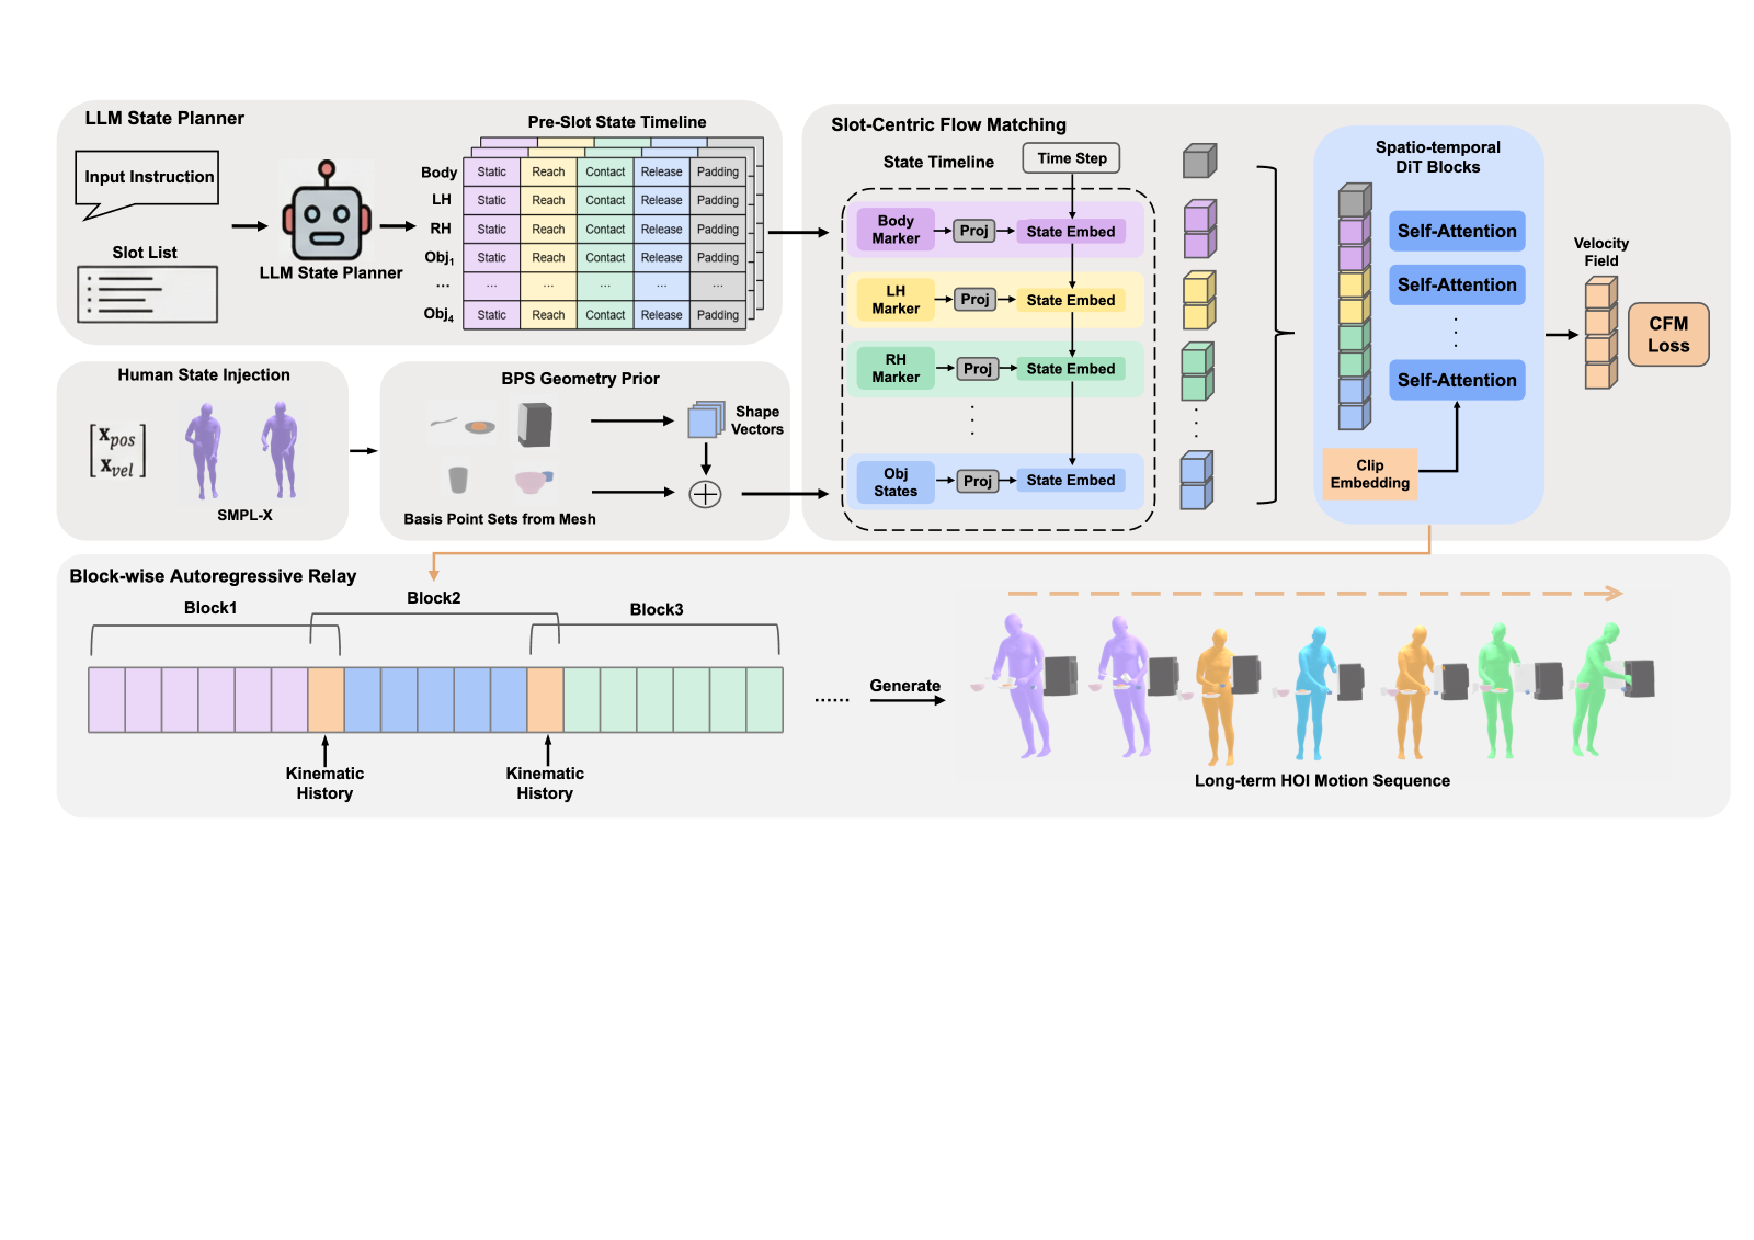
\includegraphics[width=\linewidth]{figures/framework.pdf}
  \caption{\textbf{Overview of CRR-Flow.}
The framework consists of three components.
\textbf{(a)}~An LLM-based State Planner parses multi-step textual instructions into a per-slot state timeline $\mathbf{S} \in \mathbb{Z}^{T_{\text{total}} \times 7}$, assigning discrete physical phases (Static, Reach, Contact, Release, Padding) to the body, each hand, and up to four objects.
\textbf{(b)}~A Slot-Centric Flow Matching module tokenizes the scene into dedicated spatial tokens (body, left hand, right hand, and objects), each projected independently and augmented with its scheduled state embedding.
\textbf{(c)}~A Block-wise Autoregressive Relay chains successive generation windows: the last $K$ frames of each block serve as the kinematic history for the next, ensuring continuous position and velocity across primitive boundaries.}
  \label{fig:framework}
\end{figure*}


%% ============================================================
%% 3. METHOD
%% ============================================================
\section{Method}
\label{sec:method}

Given a natural language instruction $P$ describing a manipulation task (potentially multi-sentence), our goal is to generate a temporally coherent human-object interaction motion $\mathcal{M} \in \mathbb{R}^{T \times 534}$ depicting a full-body human manipulating one or more objects. As shown in ~\cref{fig:framework}, our framework \textbf{CRR-Flow} (Contact-Release-Reach State-Aware Flow) consists of three stages: (1)~an LLM-based \emph{State Planner} that translates text into per-slot physical state timelines (\cref{sec:state_planner}), (2)~a \emph{Slot-Centric Diffusion Transformer} that generates motions conditioned on states, text, and object geometry via flow matching (\cref{sec:slot_dit}), and (3)~a \emph{Block-wise Autoregressive Relay} that extends generation to arbitrary horizons through overlapping kinematic history windows (\cref{sec:autoreg}).

\subsection{State Planning: Text to Physical State Maps}
\label{sec:state_planner}
Human-object manipulation can be decomposed into a finite set of \emph{physical interaction states}. For hands, these are: \textsc{Static} (idle), \textsc{Reach} (approaching the target), \textsc{Grasped} (holding), \textsc{Interacting} (performing a tool action), and \textsc{Release} (withdrawing). We group \textsc{Grasped} and \textsc{Interacting} under the umbrella term \emph{Contact}, so the three coarse phases motivating the CRR acronym---Contact, Reach, Release---map onto five fine-grained labels used internally. Objects transition between \textsc{Static}, \textsc{Grasped}, and \textsc{Interacting}, while unused object slots are marked \textsc{Padding}.
\paragraph{Per-slot state labels.}
For each frame $t$, we define a state vector $\mathbf{s}_t \in \{0,1,2,3,4,5\}^7$ across 7 slots: body, left hand, right hand, and up to 4 objects. The body slot is always labeled \textsc{Static}, indicating that no hand-object contact phase applies to it; the body itself can still undergo continuous kinematic motion such as reaching, leaning, or stepping. This yields a state timeline $\mathbf{S} \in \mathbb{Z}^{T \times 7}$ that specifies \emph{when} each slot should act, decoupling temporal structure from continuous motion generation.
\paragraph{Ground-truth state extraction.}
During training, state labels are computed automatically from motion capture data using a Schmitt trigger contact detector with hysteresis:
\begin{equation}
    c_t = \begin{cases}
        \text{true} & \text{if } d_t < \delta_{\text{on}} \text{ (trigger)} \\
        \text{false} & \text{if } d_t > \delta_{\text{off}} \text{ (release)} \\
        c_{t-1} & \text{otherwise (deadzone)}
    \end{cases}
    \label{eq:schmitt}
\end{equation}
where $d_t$ is the minimum fingertip-to-object distance at frame $t$, $\delta_{\text{on}} = 1.5$~cm, and $\delta_{\text{off}} = 3.0$~cm. The deadzone between thresholds prevents contact chatter at boundaries. A majority-vote filter (window size 5) further smooths isolated state transitions.
Hand-object binding is determined from task annotations: the primitive's \texttt{obj\_lh} and \texttt{obj\_rh} fields specify which hand manipulates which object, while the action topology (triadic vs.\ dyadic) determines whether secondary objects receive \textsc{Interacting} labels.


\paragraph{LLM-based state inference.}
% <<<CHANGELOG-FIX6>>> Reframed: core contribution is state representation + injection, not the LLM.
% <<<CHANGELOG-FIX7>>> Clarified frame count determination: fixed primitive length, not inferred by LLM.
At test time, when ground-truth states are unavailable, we query a large language model to produce structured segment-level state annotations. The prompt is grounded in the predefined state vocabulary described above and asks the model to assign one of the five interaction phases to each slot for every primitive segment (prompt details are provided in the supplementary material). Because each primitive has a fixed length of $L{=}180$ generation frames plus a $K{=}20$-frame history window, the temporal structure is explicitly defined rather than inferred by the language model; the LLM only determines \emph{which} state applies to \emph{which} slot within each segment. Given the instruction and slot list, the LLM outputs a state timeline:
\begin{equation}
    \text{LLM}(P, \text{entities}) \rightarrow \mathbf{S} \in \mathbb{Z}^{T_{\text{total}} \times 7}.
    \label{eq:llm_planner}
\end{equation}
During autoregressive generation (\cref{sec:autoreg}), the system slices the corresponding $T$-frame segment from $\mathbf{S}$ for each generation block, so that all blocks share a globally consistent state timeline rather than invoking the LLM independently per block.
We note that the core contribution is the state representation itself---the per-slot phase vocabulary, the Schmitt-trigger extraction procedure, and the injection mechanism described in \cref{sec:slot_dit}---rather than the choice of language model used at inference time.



\subsection{Slot-Centric Flow Matching DiT}
\label{sec:slot_dit}

\paragraph{Motion representation.}
We represent the human body using \textbf{77 surface markers} extracted from SMPL-X~\cite{pavlakos2019expressive} mesh vertices, following the SSM67 protocol~\cite{xu2024interdiff} augmented with 10 fingertip markers. The markers are partitioned into three groups: body (50 markers, 150D), left hand (14 markers, 42D), and right hand (13 markers, 39D), totaling 231D of positional features.

Each object is represented by a 9D pose vector (3D translation + 6D rotation), with up to 4 object slots. Object geometry is encoded using \textbf{Basis Point Sets (BPS)}~\cite{prokudin2019efficient}: 1024 Fibonacci-distributed basis points, each storing the scalar distance to the nearest object surface point, yielding a static 1024D shape embedding per object.

\paragraph{Velocity features.}
For each positional feature, we compute the first-order temporal difference $\mathbf{v}_t = \mathbf{x}_t - \mathbf{x}_{t-1}$ \emph{after} temporal downsampling to the target frame rate. This produces a 267D velocity vector with the same layout as positions. The full dynamic feature is the concatenation $[\mathbf{x}_{\text{pos}}; \mathbf{x}_{\text{vel}}] \in \mathbb{R}^{534}$ per frame. After concatenation, the per-slot dynamic dimensions are: body $150{\times}2{=}300$D, left hand $42{\times}2{=}84$D, right hand $39{\times}2{=}78$D, and each object $9{\times}2{=}18$D.

\paragraph{Slot tokenization.}
Unlike prior methods that treat the full feature vector as a monolithic token, we decompose it into \textbf{7 slot tokens} per frame, each processed through a dedicated input projection:
\begin{align}
    \mathbf{h}_{\text{body}} &= W_{\text{body}} \, \mathbf{x}_{\text{body}} \in \mathbb{R}^D, \quad (300 \rightarrow 512) \\
    \mathbf{h}_{\text{lh}} &= W_{\text{lh}} \, \mathbf{x}_{\text{lh}} \in \mathbb{R}^D, \quad (84 \rightarrow 512) \\
    \mathbf{h}_{\text{rh}} &= W_{\text{rh}} \, \mathbf{x}_{\text{rh}} \in \mathbb{R}^D, \quad (78 \rightarrow 512) \\
    \mathbf{h}_{\text{obj}_i} &= W_{\text{obj}} \, [\mathbf{x}_{\text{obj}_i}; \mathbf{b}_i] \in \mathbb{R}^D, \quad (1042 \rightarrow 512)
    \label{eq:slot_proj}
\end{align}
where $\mathbf{b}_i \in \mathbb{R}^{1024}$ is the BPS embedding concatenated to the object's dynamic features before projection. Body, left hand, and right hand each use a separate projection because their marker layouts and dimensionalities differ. All four object slots share $W_{\text{obj}}$ because objects occupy a common feature space (18D dynamics $+$ 1024D BPS geometry); sharing the projection improves generalization across varying object instances while reducing parameter count.
Since object geometry is time-invariant, $\mathbf{b}_i$ is kept \emph{noise-free} throughout the flow matching process: only the 18D dynamic component (position + velocity) of each object undergoes the noise schedule, while the static shape descriptor enters as clean context.


\paragraph{Per-slot state injection.}
State labels are embedded and added \emph{directly} to the corresponding slot token, not broadcast globally:
\begin{equation}
    \mathbf{h}_e \leftarrow \mathbf{h}_e + \text{StateEmbed}(\mathbf{s}_{t,e}), \quad e \in \{\text{lh}, \text{rh}, \text{obj}_1, \ldots, \text{obj}_4\}.
    \label{eq:state_inject}
\end{equation}
The body slot receives no state injection (always \textsc{Static}). Compared with global conditioning, where all entities share a single state vector, per-slot injection removes the ambiguity of which hand is reaching and which object is being grasped at each frame.

\paragraph{Spatio-temporal self-attention.}
The 7 slot tokens per frame are stacked with dual positional encodings---sinusoidal temporal PE and learned slot PE---then flattened to a sequence of $T \times 7$ tokens:
\begin{equation}
    \mathbf{H} = \text{Flatten}\left(\mathbf{h}_{t,e} + \text{PE}_{\text{time}}(t) + \text{PE}_{\text{slot}}(e)\right) \in \mathbb{R}^{(T \cdot 7) \times D}.
    \label{eq:flatten}
\end{equation}
This sequence is processed by $L{=}8$ DiT blocks~\cite{peebles2023scalable} with AdaLN-Zero~\cite{peebles2023scalable} modulation and FlashAttention-2~\cite{dao2023flashattention2}. The joint spatio-temporal attention allows each slot token at frame $t$ to attend to all other entities across frames, capturing inter-slot coordination.

Unused object slots (\textsc{Padding}) are masked via key padding so that the model does not generate motion for absent objects.

\paragraph{Conditioning.}
The global condition vector fuses the diffusion timestep embedding with a CLIP~\cite{radford2021learning} ViT-B/32 text embedding:
\begin{equation}
    \mathbf{c} = \text{MLP}([\text{TimestepEmbed}(t); W_{\text{text}}\,\text{CLIP}(P)]).
    \label{eq:condition}
\end{equation}
Classifier-free guidance~\cite{ho2022classifier} is enabled by randomly replacing the text embedding with a zero vector with probability 0.1 during training. State labels and BPS embeddings are \emph{not} dropped, as they provide hard structural constraints (hand-object binding and object geometry) required for physically valid generation. The guidance scale and other inference hyperparameters are reported in \cref{sec:experiments}.

\paragraph{Output projections.}
After the transformer, tokens are unflattened and projected back to raw dimensions through per-slot output layers. The output predicts only the \emph{dynamic} components (position + velocity); BPS geometry is excluded from the prediction target since it is static:
\begin{equation}
    \hat{\mathbf{v}} = [W_{\text{body}}^{\text{out}}\,\mathbf{h}_{\text{body}}; W_{\text{lh}}^{\text{out}}\,\mathbf{h}_{\text{lh}}; W_{\text{rh}}^{\text{out}}\,\mathbf{h}_{\text{rh}}; W_{\text{obj}}^{\text{out}}\,\mathbf{h}_{\text{obj}_1}; \ldots] \in \mathbb{R}^{534}.
    \label{eq:output}
\end{equation}

\paragraph{Flow matching formulation.}
We adopt Conditional Flow Matching (CFM)~\cite{lipman2023flow} as the generative backbone. CFM learns a velocity field $v_\theta$ that transports samples from a Gaussian prior $\mathbf{x}_0 \sim \mathcal{N}(0, \mathbf{I})$ to the data distribution along the linear interpolation path $\mathbf{x}_t = (1{-}t)\mathbf{x}_0 + t\,\mathbf{x}_1$. The network is trained to predict the target velocity $\mathbf{u}_t = \mathbf{x}_1 - \mathbf{x}_0$ given the noised sample $\mathbf{x}_t$, the flow timestep $t$, the state timeline $\mathbf{S}$, the text condition $\mathbf{c}$, and the BPS embeddings $\mathbf{B}$. The concrete training objective, which incorporates history-conditioned masking, is presented in \cref{sec:autoreg}.


\begin{table*}[t]
  \caption{\textbf{Main results on OakInk2.}
  All generation quality metrics use a motion--text evaluator fine-tuned on OakInk2.
  Marker MSE is computed directly against ground-truth marker positions.
  Best results in \textbf{bold}.
  $\downarrow$: lower is better; $\uparrow$: higher is better.
  $^\dagger$: body-only, no hands or objects.
  $^\ddagger$: trained on OakInk2 primitive-level data.}
  \label{tab:main_oakink2}
  \centering
  \small
  \begin{tabular}{@{}l|ccc|cccc|c@{}}
    \toprule
    \multirow{2}{*}{Method} & \multicolumn{3}{c|}{R-Precision} & \multicolumn{4}{c|}{Generation Quality} & Reconstruction \\
    & Top-1 $\uparrow$ & Top-2 $\uparrow$ & Top-3 $\uparrow$ & FID $\downarrow$ & Matching $\downarrow$ & Diversity $\uparrow$  & MultiMod $\uparrow$ & Marker MSE $\downarrow$ \\
    \midrule
    PriorMDM DoubleTake$^\dagger$& 0.410 & 0.519 & 0.585 & 15.701 & 13.836 & \textbf{5.302}  & \textbf{5.326} & --- \\
    InterAct HOIDiff$^\ddagger$ & 0.641 & 0.796 & 0.910 & 2.821 & 5.919 & 1.494  & 2.233 & 0.0385 \\
    \midrule
    CRR-Flow w/o AR & 0.672 & 0.859 & 0.940 & 0.445 & 3.370& 1.407  & 1.923 & 0.0202 \\
    CRR-Flow (Ours) & \textbf{0.720} & \textbf{0.891} & \textbf{0.953}& \textbf{0.438} & \textbf{3.010} & 1.256  & 0.681 & \textbf{0.0140} \\
    \bottomrule
  \end{tabular}
\end{table*}



\subsection{Block-wise Autoregressive Relay}
\label{sec:autoreg}

To extend generation beyond the fixed $T{=}200$-frame window to long-horizon motions spanning multiple action phases, we employ a block-wise autoregressive strategy.

\paragraph{History-target decomposition.}
During training, each window of $T{=}200$ frames is decomposed into:
\begin{itemize}
    \item \textbf{Kinematic history} $\mathbf{X}_{\text{hist}}$: the first $K{=}20$ frames (2 seconds at 10~FPS) are kept \emph{noise-free}, providing a clean conditioning context with ground-truth positions and velocities.
    \item \textbf{Generation target} $\mathbf{X}_{\text{target}}$: the remaining $L{=}180$ frames receive flow matching noise and are the prediction target.
\end{itemize}
To bridge the distribution gap between training (where $\mathbf{X}_{\text{hist}}$ contains ground-truth motion) and inference (where the first block starts from a static rest pose), we employ a mixed sampling strategy: 20\% of training windows use a \emph{cold-start} history in which $\mathbf{X}_{\text{hist}}$ is set to a repeated rest pose with zero velocity. This exposes the model to both in-motion relay and static-start conditions during training.

The history and noised target are concatenated along the temporal axis:
\begin{equation}
    \mathbf{x}_t^{\text{full}} = [\mathbf{X}_{\text{hist}}; \mathbf{x}_t^{\text{target}}] \in \mathbb{R}^{T \times 534},
    \label{eq:autoreg_concat}
\end{equation}
and the loss mask zeroes gradients for the $K$ history frames. The training objective is:
\begin{equation}
    \mathcal{L} = \mathbb{E}_{t, \mathbf{x}_0, \mathbf{x}_1}\left[\left\| v_\theta(\mathbf{x}_t^{\text{full}}, t, \mathbf{S}, \mathbf{c}, \mathbf{B}) - \mathbf{u}_t \right\|^2 \cdot \mathbf{M}_{\text{target}}\right],
    \label{eq:autoreg_loss}
\end{equation}
where $\mathbf{u}_t = \mathbf{x}_1 - \mathbf{x}_0$ is the target velocity field, and $\mathbf{M}_{\text{target}}$ is 0 for the first $K$ frames and 1 for the remaining $L$ frames. 



The history and noised target are concatenated along the temporal axis:
\begin{equation}
    \mathbf{x}_t^{\text{full}} = [\mathbf{X}_{\text{hist}}; \mathbf{x}_t^{\text{target}}] \in \mathbb{R}^{T \times 534},
    \label{eq:autoreg_concat}
\end{equation}
and the loss mask zeroes gradients for the $K$ history frames, yielding the actual training objective:
\begin{equation}
    \mathcal{L}_{\text{AR}} = \mathbb{E}\left[\left\| v_\theta(\mathbf{x}_t^{\text{full}}, t, \mathbf{S}, \mathbf{c}, \mathbf{B}) - \mathbf{u}_t \right\|^2 \cdot \mathbf{M}_{\text{target}}\right],
    \label{eq:autoreg_loss}
\end{equation}
where $\mathbf{M}_{\text{target}}$ is 0 for the first $K$ frames and 1 for the remaining $L$ frames. This objective is used throughout training and the standard $\mathcal{L}_{\text{FM}}$ corresponds to the special case $K{=}0$.

\paragraph{Sliding window relay.}
For long-horizon generation ($T > 200$), CRR-Flow chains multiple generation windows:
\begin{enumerate}
    \item \textbf{Initialization}: $\mathbf{X}_{\text{hist}}$ is set to the rest pose with zero velocity for the first segment.
    \item \textbf{Generation}: The model generates $L{=}180$ frames conditioned on $\mathbf{X}_{\text{hist}}$ and the current state/text instruction.
    \item \textbf{Relay}: The \emph{last} $K$ frames of the generated segment become the new $\mathbf{X}_{\text{hist}}$, and the next $T$-frame slice of the global state timeline $\mathbf{S}$ is loaded as the condition for the next block.
\end{enumerate}
Because each block inherits the terminal kinematic state of its predecessor, position and velocity remain continuous across segment boundaries---e.g., the hand's velocity at the end of a \textsc{Reach} phase carries over into the subsequent \textsc{Grasped} phase uninterruptedly.

\paragraph{Distribution gap at inference time.}
From the second block onward, the history window contains model-generated motion rather than ground-truth data, introducing a distribution gap relative to training. In practice, this gap does not lead to severe error accumulation for two reasons. First, the history window is short ($K{=}20$ frames), which limits the temporal horizon over which conditioning errors can propagate; each block effectively ``resets'' its context from a narrow window rather than from the entire preceding sequence. Second, the flow matching objective is empirically robust to small perturbations in the conditioning signal, as the velocity field prediction depends primarily on the local kinematic state (position and velocity) rather than on fine-grained details of the conditioning trajectory. The long-horizon evaluation in \cref{sec:long_horizon} confirms this: Marker MSE degrades by only 8.6\% from single-segment quality across chains of up to 4 segments.


%% ============================================================
%% 4. EXPERIMENTS
%% ============================================================

\section{Experiments}
\label{sec:experiments}

\begin{table}[t]
  \caption{\textbf{Ablation study on OakInk2.} Components are removed cumulatively from the full model. $\Delta$~MSE: relative change in Marker MSE vs.\ the full model.}
  \label{tab:ablation}
  \centering
  \small
  \begin{tabular}{@{}lccc@{}}
    \toprule
    Configuration & M-MSE $\downarrow$ & FID $\downarrow$ & $\Delta$ MSE \\
    \midrule
    \textbf{CRR-Flow} (full) & \textbf{0.0140} & \textbf{0.438} & --- \\
    \quad w/o Autoregressive & 0.0202 & 0.445 & $+$44.3\% \\
    \quad w/o Vel $+$ BPS & 0.0248 & 0.585 & $+$77.1\% \\
    \bottomrule
  \end{tabular}
\end{table}


\subsection{Datasets}
\label{sec:datasets}

\paragraph{OakInk2~\cite{zhan2024oakink2}.}
A long-horizon human-object interaction dataset captured with SMPL-X~\cite{pavlakos2019expressive} body tracking and multi-object 6DoF annotations.
We extract 963 super-segments from 627 complex sequences by merging adjacent primitives with temporal gaps ${\leq}\,300$ frames.
Each segment undergoes boundary expansion (${\pm}60$ frames), downsampling from 30 to 10~FPS, and uniform subsampling to $T{=}200$ frames, yielding 534D dynamic features (267D positions $+$ 267D velocities) with up to 4 object slots.
Per-slot state labels $[T, 7]$ are computed via Schmitt-trigger contact detection ($\delta_\text{on}{=}1.5$~cm, $\delta_\text{off}{=}3.0$~cm) with majority-vote smoothing. We additionally evaluate on HIMO~\cite{himo2024} to validate generalizability across diverse spatial layouts; results are reported in the Supplementary Material.
% \paragraph{OakInk2~\cite{zhan2024oakink2} (Primary Benchmark).}
% A bimanual hand-object manipulation dataset captured with SMPL-X~\cite{pavlakos2019expressive} body tracking and multi-object 6DoF annotations.
% We extract 963 super-segments from 627 complex sequences by merging adjacent primitives with temporal gaps ${\leq}\,300$ frames.
% Each segment undergoes boundary expansion (${\pm}60$ frames), downsampling from 30 to 10~FPS, and uniform subsampling to $T{=}200$ frames, yielding 534D dynamic features (267D positions $+$ 267D velocities) with up to 4 object slots.
% Per-slot state labels $[T, 7]$ are computed via Schmitt-trigger contact detection ($\delta_\text{on}{=}1.5$~cm, $\delta_\text{off}{=}3.0$~cm) with majority-vote smoothing. We additionally evaluate on HIMO~\cite{himo2024} to validate generalizability across diverse spatial layouts; results are reported in the Supplementary Material.
\paragraph{GRAB~\cite{taheri2020grab}.}
A single-hand grasping dataset with 1{,}335 sequences across 10 subjects and 51 objects.
Raw SMPL-X parameters at 120~FPS are downsampled to 30~FPS.
State labels are derived from ground-truth per-vertex contact annotations on all 10{,}475 SMPL-X vertices, providing precise contact supervision.

\begin{table}[t]
  \caption{\textbf{Long-horizon generation on OakInk2.} Each row chains multiple segments via $K{=}20$-frame history relay. Single-segment Marker MSE is 0.014 for reference.}
  \label{tab:long_horizon}
  \centering
  \small
  \begin{tabular}{@{}lccc@{}}
    \toprule
    Task & Segments & Frames (Duration) & M-MSE $\downarrow$ \\
    \midrule
    Rearrange plate & 4 & 740 (74s) & 0.0116 \\
    Scoop cheese  & 3 & 560 (56s) & 0.0185 \\
    Insert lightbulb & 3 & 560 (56s) & 0.0139 \\
    Take donut & 3 & 560 (56s) & 0.0167 \\
    \midrule
    \textbf{Average} & 3.25 & 605 (60.5s) & \textbf{0.0152} \\
    \bottomrule
  \end{tabular}
\end{table}



\subsection{Baselines}
\label{sec:baselines}

We compare against two representative methods that address different aspects of the problem:

\paragraph{InterAct HOIDiff~\cite{xu2025interact}.}
A text-conditioned diffusion model for single-segment HOI generation.
HOIDiff employs a dual transformer backbone with PointNet2/BPS object encoding.
Since HOIDiff~\cite{2025_hoidiff} is designed for single-primitive generation, we train it from scratch on OakInk2 \emph{primitive-level} data following the original preprocessing.
It generates 962D motions but lacks per-slot state conditioning and autoregressive capability.

\paragraph{PriorMDM~\cite{shafir2024priormdm}.}
A long-horizon body motion composition method that chains motion segments via a two-pass handshake-and-blend strategy.
PriorMDM uses a pre-trained MDM~\cite{tevet2023human} backbone on HumanML3D~\cite{guo2022generating} (14K sequences, 263D body-only).
It generates 22 body joints without hand articulation or object interaction and serves as a long-horizon body-only baseline.


\subsection{Evaluation Metrics}
\label{sec:metrics}

We train a motion--text evaluator on OakInk2 following the contrastive learning protocol of InterAct~\cite{xu2025interact}.
From this evaluator we compute:
\textbf{R-Precision}~(Top-1/2/3): retrieval accuracy of the ground-truth text among 32 candidates given the motion embedding;
\textbf{FID}~\cite{heusel2017gans}: Fr\'{e}chet Inception Distance between generated and real motion feature distributions;
\textbf{Matching Score}: L2 distance between paired text and motion embeddings (lower is better);
\textbf{Diversity}: average pairwise L2 distance in the motion embedding space;
\textbf{MultiModality}: variance of motion embeddings generated from the same text prompt.
For reconstruction, we report \textbf{Marker MSE} (mean squared error of 77 marker positions vs.\ ground truth).



\subsection{Main Results on OakInk2}
\label{sec:main_results}
% \Cref{tab:main_oakink2} compares CRR-Flow against baselines on OakInk2 dataset.
\paragraph{CRR-Flow Outperforms Baselines Across All Core Metrics.} In ~\cref{tab:main_oakink2},
CRR-Flow achieves the best R-Precision, FID, Matching Score, and Marker MSE.
Compared with InterAct HOIDiff, R-Precision Top-1 improves by 12.3\% (0.720 vs.\ 0.641), FID drops by 84.5\% (0.438 vs.\ 2.821), Matching Score improves by 49.1\% (3.010 vs.\ 5.919), and Marker MSE decreases by 63.6\% (0.014 vs.\ 0.039).
PriorMDM, trained on HumanML3D body-only data, scores poorly on R-Precision (0.410) and FID (15.701), confirming that body-only models do not transfer to the HOI domain.
PriorMDM does achieve the highest Diversity (5.302) and MultiModality (5.326), reflecting the broader kinematic variation in full-body locomotion compared with the constrained manipulation tasks in OakInk2.

\paragraph{Autoregressive Relay Improves Fidelity at a Diversity Cost.}
The autoregressive model improves over the non-autoregressive variant on R-Precision (0.720 vs.\ 0.672), FID (0.438 vs.\ 0.445), Matching Score (3.010 vs.\ 3.370), and Marker MSE (0.014 vs.\ 0.020), with a 30.7\% reduction in reconstruction error.
The history window grounds generation on the preceding kinematic context, producing motions that are more faithful to both the text and the physical state.
The cost is reduced MultiModality (0.681 vs.\ 1.923): conditioning on a specific kinematic history narrows the space of plausible continuations, yielding less variation across samples from the same prompt.
Diversity also decreases (1.256 vs.\ 1.407), though the effect is smaller.
\Cref{fig:comparison} illustrates these differences on a representative primitive: PriorMDM produces body-only motion but lacks hand articulation entirely, while InterAct HOIDiff generates human-object motion with noticeable penetration artifacts.
CRR-Flow maintains finger-object conformity from the initial grasp through placement.

\begin{table}[t]
  \caption{\textbf{Contact evaluation on GRAB.} Both methods trained on GRAB with ground-truth per-vertex contact labels. Evaluated on 28 overlapping test sequences.}
  \label{tab:contact_eval}
  \centering
  \small
  \begin{tabular}{@{}lccc@{}}
    \toprule
    Method & Precision $\uparrow$ & Recall $\uparrow$ & F1 $\uparrow$ \\
    \midrule
    InterAct HOIDiff~\cite{xu2025interact} & 0.254 & 0.113 & 0.129 \\
    \textbf{CRR-Flow (Ours)} & \textbf{0.310} & \textbf{0.255} & \textbf{0.251} \\
    \bottomrule
  \end{tabular}
\end{table}


\subsection{Ablation Study}
\label{sec:ablation}

We ablate two key design decisions: the autoregressive relay and the velocity/BPS input features in \cref{tab:ablation}.
Starting from the full model, we remove the autoregressive relay, then additionally strip velocity features and BPS geometry.

\paragraph{Autoregressive Relay ($-$30.7\% MSE, $-$1.6\% FID)}
Removing the block-wise autoregressive strategy ($K{=}20$ history frames) increases Marker MSE from 0.014 to 0.020 and FID from 0.438 to 0.445.
The history window provides a kinematic anchor: rather than generating from pure noise, the model conditions on 2 seconds of established motion, grounding body position, velocity, and spatial relationships.
This is the single largest component contribution.
 
\paragraph{Velocity Features and BPS Geometry ($-$18.5\% MSE)}
Further removing velocity features and BPS object geometry (reducing input to 267D positions only) increases Marker MSE from 0.020 to 0.025 and FID from 0.445 to 0.585.
Velocity provides an explicit inductive bias for temporal dynamics, and BPS geometry enables shape-aware manipulation through the object projection layer (1042D $\to$ 512D), which compresses both dynamic pose (18D) and static shape (1024D) into a single slot token.


%% ============================================================
%% FIGURE: Comparison with Baselines
%% ============================================================
\begin{figure*}[t]
  \centering
  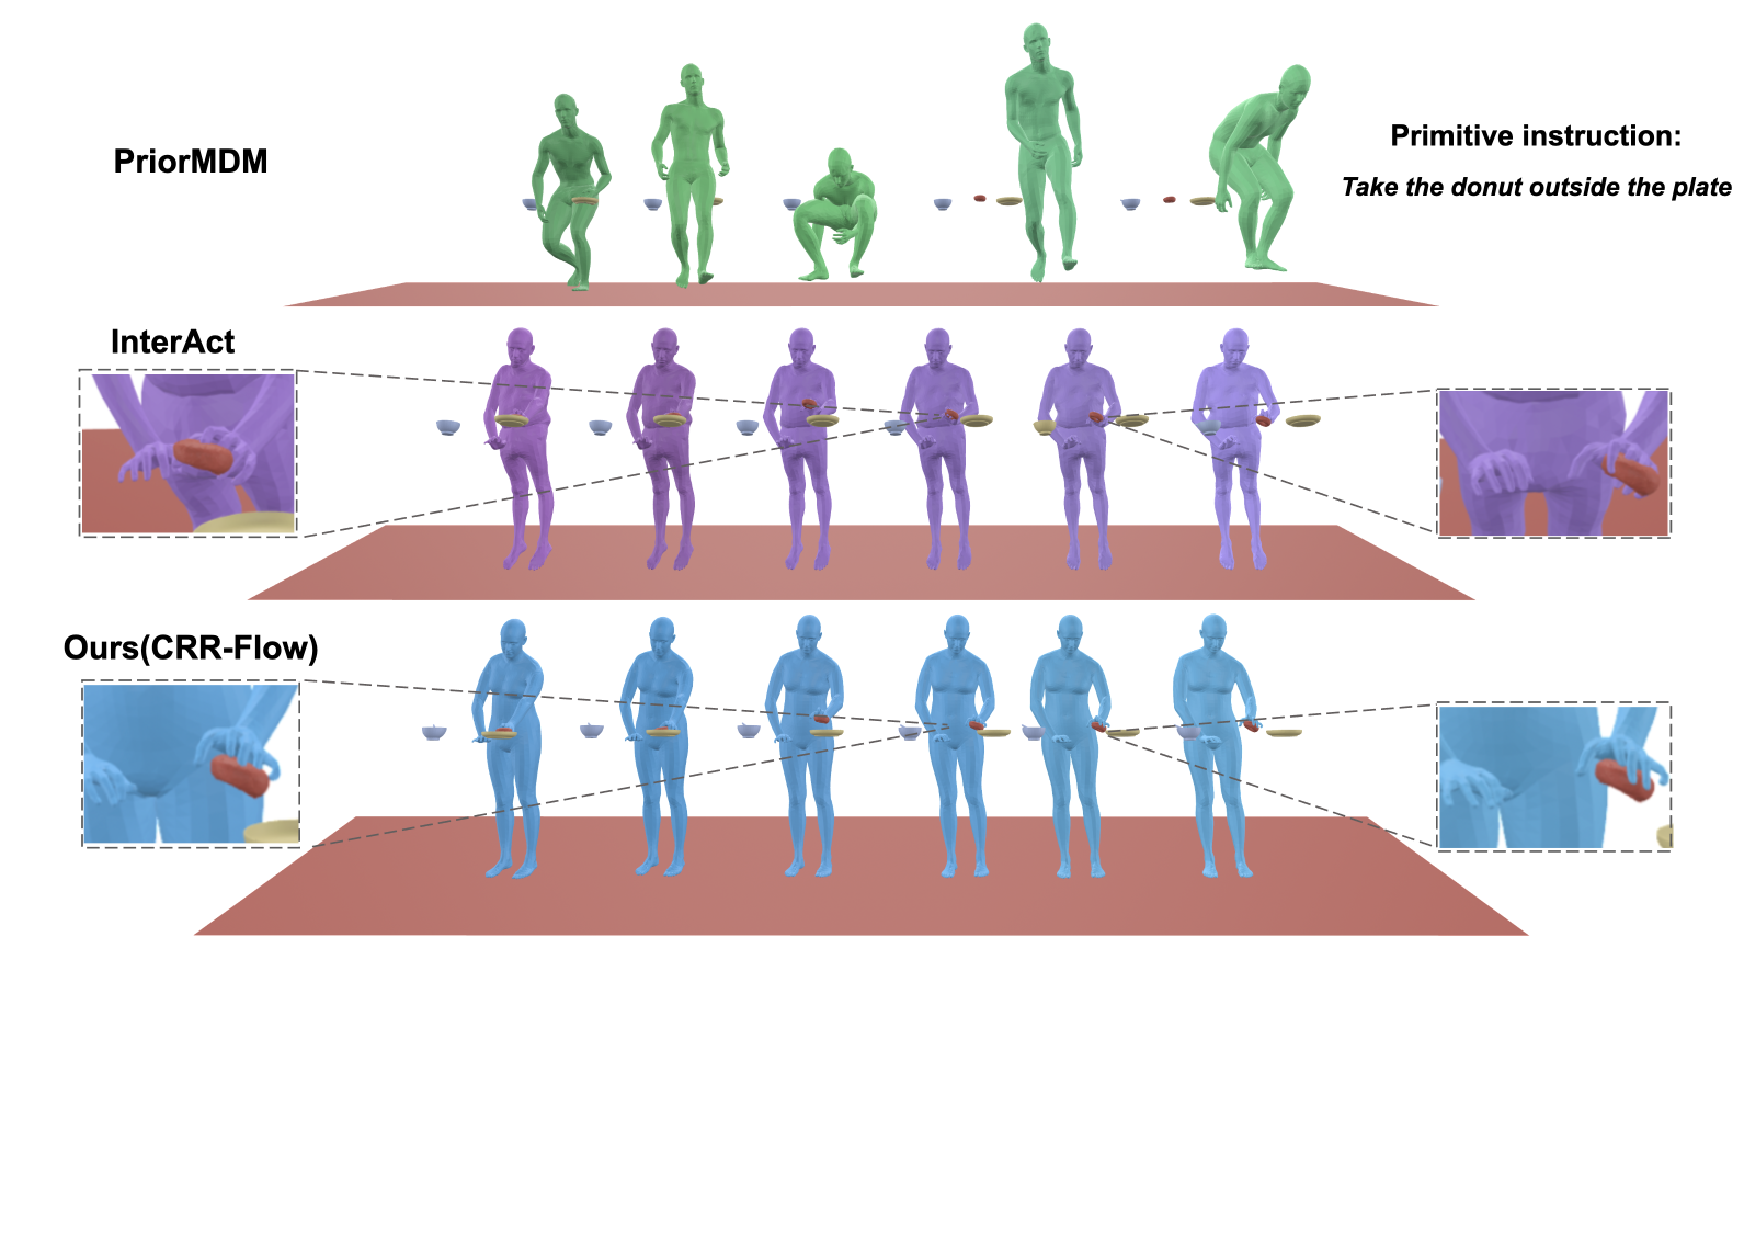
\includegraphics[width=\linewidth]{./figures/comparison.pdf}
  \caption{\textbf{Qualitative comparison on a single-primitive task}.
  PriorMDM (top, green) generates body-only motion without hand articulation or object dynamics; objects remain static throughout.
  InterAct HOIDiff (middle, purple) produces human-object motion but suffers from hand-object penetration---the close-up insets show fingers passing through the donut surface.
  CRR-Flow (bottom, blue) generates a coherent reach-grasp sequence with plausible finger-object contact throughout.}
  \Description{Three-row qualitative comparison. Top row: PriorMDM generates green body meshes with no hand detail and static objects. Middle row: InterAct generates purple meshes with hands but visible hand-object penetration shown in zoomed insets. Bottom row: CRR-Flow generates blue meshes with consistent hand-object contact visible in zoomed insets at both grasp initiation and object placement.}
  \label{fig:comparison}
\end{figure*}


 
\subsection{Long-Horizon Autoregressive Generation}
\label{sec:long_horizon}

We evaluate CRR-Flow on multi-segment chains from the OakInk2 test set, where consecutive super-segments from the same complex task are chained by relaying the last $K{=}20$ frames as history for the next block in \cref{tab:long_horizon}.

The average long-horizon Marker MSE (0.015) degrades by only 8.6\% from single-segment quality (0.014), despite generating up to 740 frames (74 seconds) of continuous manipulation.
The longest chain (\emph{Rearrange plate}, 4 segments) achieves the lowest MSE (0.012), while the hardest chain (\emph{Scoop cheese}, 0.019) involves complex bimanual coordination with tool use.

\subsection{Contact Evaluation on GRAB}
\label{sec:contact_eval}
 
To evaluate contact quality directly, we train both CRR-Flow and InterAct HOIDiff on GRAB~\cite{taheri2020grab}, which provides ground-truth per-vertex contact annotations on the SMPL-X mesh.
Unlike OakInk2, where contact labels are approximated from distance thresholds, GRAB enables precise vertex-level evaluation.
We report Precision, Recall, and F1 on the 28 overlapping test sequences in \cref{tab:contact_eval}.
 
CRR-Flow achieves a Contact F1 of 0.251 vs.\ 0.129 for InterAct HOIDiff---a 94.6\% relative improvement.
The gain is driven primarily by Recall (0.255 vs.\ 0.113): per-slot state injection signals when each hand should be in contact, so the model produces grasps at the correct frames rather than missing contact windows.
Precision also improves (0.310 vs.\ 0.254), indicating that the generated contacts land at plausible surface locations.
 
 
% \subsection{Cross-Dataset Evaluation}
% \label{sec:cross_dataset}

% To assess the generality of our slot-centric architecture, we train CRR-Flow on GRAB and OMOMO in \cref{tab:cross_dataset}.
% GRAB provides ground-truth per-vertex contact annotations, enabling reliable Contact F1 evaluation---unlike OakInk2, where contact labels are approximated from distance thresholds.

% \begin{table}[t]
%   \caption{\textbf{Cross-dataset results.} CRR-Flow trained separately on each dataset. Contact F1 is reported only for GRAB, which provides ground-truth per-vertex contact labels.}
%   \label{tab:cross_dataset}
%   \centering
%   \small
%   \begin{tabular}{@{}lcccc|c@{}}
%     \toprule
%     Dataset & M-MSE $\downarrow$ & Obj Pos $\downarrow$ & Jitter $\downarrow$ & Obj Rot $\downarrow$ & Contact F1 $\uparrow$ \\
%     \midrule
%     OakInk2 & \textbf{0.014} & \textbf{223} & \textbf{0.006} & 91.5 & --- \\
%     GRAB & 0.069 & 383 & 0.011 & 109 & \textbf{0.190} \\
%     OMOMO & 0.386 & 1105 & 0.029 & 92.8 & --- \\
%     \bottomrule
%   \end{tabular}
% \end{table}

% On GRAB, CRR-Flow achieves a Contact F1 of 0.19, benefiting from the precise per-vertex contact supervision that enables the state conditioning mechanism to function at its full potential.
% OMOMO presents the greatest challenge: its large furniture objects (suitcases, tables) require whole-body coordination patterns fundamentally different from the fine-grained hand manipulation in OakInk2 and GRAB, resulting in substantially higher reconstruction errors.
% The slot-centric tokenization and state conditioning framework generalizes across all three datasets without architectural changes, requiring only dataset-specific preprocessing.



\subsection{Implementation Details}
\label{sec:implementation}

CRR-Flow uses a DiT backbone with latent dimension $D{=}512$, 8 transformer layers, 8 attention heads, and FFN dimension 2048, totaling 41.2M trainable parameters (excluding frozen CLIP ViT-B/32).
We train with AdamW ($\text{lr}{=}10^{-4}$, weight decay $0.01$) with gradient clipping at 1.0 and batch size 32 until convergence.
CLIP text embeddings are pre-computed and cached for memory efficiency.
Inference uses ODE integration with Euler's method (10 steps).
All experiments are conducted on NVIDIA RTX A6000 GPUs.


%% ============================================================
%% 5. CONCLUSION & Limitations and Future Work
%% ============================================================


\section{Conclusion}
\label{sec:conclusion}

We have presented CRR-Flow, a unified framework for generating long-horizon, multi-object hand-object interaction sequences from multi-step natural language instructions.
Our approach introduces three mutually reinforcing components: (1)~a per-slot physical state scheduling mechanism that translates free-form instructions into dense per-frame state matrices through an LLM-based planner, bridging semantic task understanding and kinematic generation via a shared state representation;
(2)~a slot-centric Diffusion Transformer that models the body, hands, and objects as dedicated spatial tokens with per-slot state injection and geometry-aware object encoding; and (3)~a block-wise autoregressive relay that propagates terminal kinematic history across generation blocks, maintaining continuous dynamics over thousands of frames.
Experiments on OakInk2 demonstrate that CRR-Flow reduces reconstruction error by over 30\% compared to the non-autoregressive variant and achieves long-horizon generation with only 8.6\% degradation from single-segment quality.
Contact evaluation on GRAB shows that per-slot state injection nearly doubles Contact F1 relative to InterAct HOIDiff.


\paragraph{Limitations and future work.}
% The current LLM-based state planner operates in an open-loop manner, producing the full state timeline before generation begins; errors in temporal estimation cannot be corrected mid-sequence.
% Incorporating closed-loop replanning that adapts state schedules based on intermediate generation results is a promising direction.
% Additionally, 
The Schmitt-trigger contact labels provide effective supervision for grasping tasks, extending the state vocabulary to capture finer-grained manipulation phases would broaden the range of expressible interactions.
Finally, integrating physics-based contact refinement into the generation pipeline could further improve grasp stability and reduce residual penetrations in complex bimanual scenarios.


% %%
% %% Acknowledgments
% %%
% \begin{acks}
% To be added.
% \end{acks}


%%
%% Bibliography
%%
\bibliographystyle{ACM-Reference-Format}
\bibliography{main}

\end{document}
\endinput
